\lecture{Digital Twin Applications}{16~-~01~-~2026}
%
\section{Applications in product lifecycle}
Il Digital Twin non è limitato a una singola fase, ma attraversa e integra diverse fasi del ciclo di vita del prodotto.
%
\paragraph{Design phase} Permette una progettazione più reattiva ed efficiente attraverso la modellazione basata sulla fisica. Consente la pre-verifica concettuale e la predizione delle performance prima della produzione effettiva e aiuta a gestire l'incertezza e la mancanza di dati fisici per eliminare potenziali guasti.
%
\paragraph{Production phase} Lo spazio virtuale rispecchia quello fisico in tempo reale, permettendo il controllo dei comportamenti fisici: migliora l'affidabilità, la flessibilità e la predittività (forecasting accurato). Ottimizza anche i consumi energetici e il throughput, permettendo aggiustamenti tempestivi.
%
\paragraph{Maintenance phase} È storicamente il primo campo di applicazione e quello che riceve più attenzione, combina dati dei sensori e dati storici per la predizione dei guasti. Fa utilizzo di Machine Learning e modellazione multi-fisica per aumentare l'affidabilità e prolungare la vita delle macchine.

Ovviamente il valore aggiunto sta nell'integrazione continua delle fasi e dei dati: l'esperienza storica del ciclo di vita viene usata nel design per simulazioni accurate; viceversa, gli artefatti digitali del design vengono aggiustati durante il servizio per la manutenzione.
Vedi figura \ref{fig:app-intro1} e \ref{fig:app-intro2} a riguardo.
\begin{figure}
    \centering
    \begin{subfigure}{0.9\linewidth}
        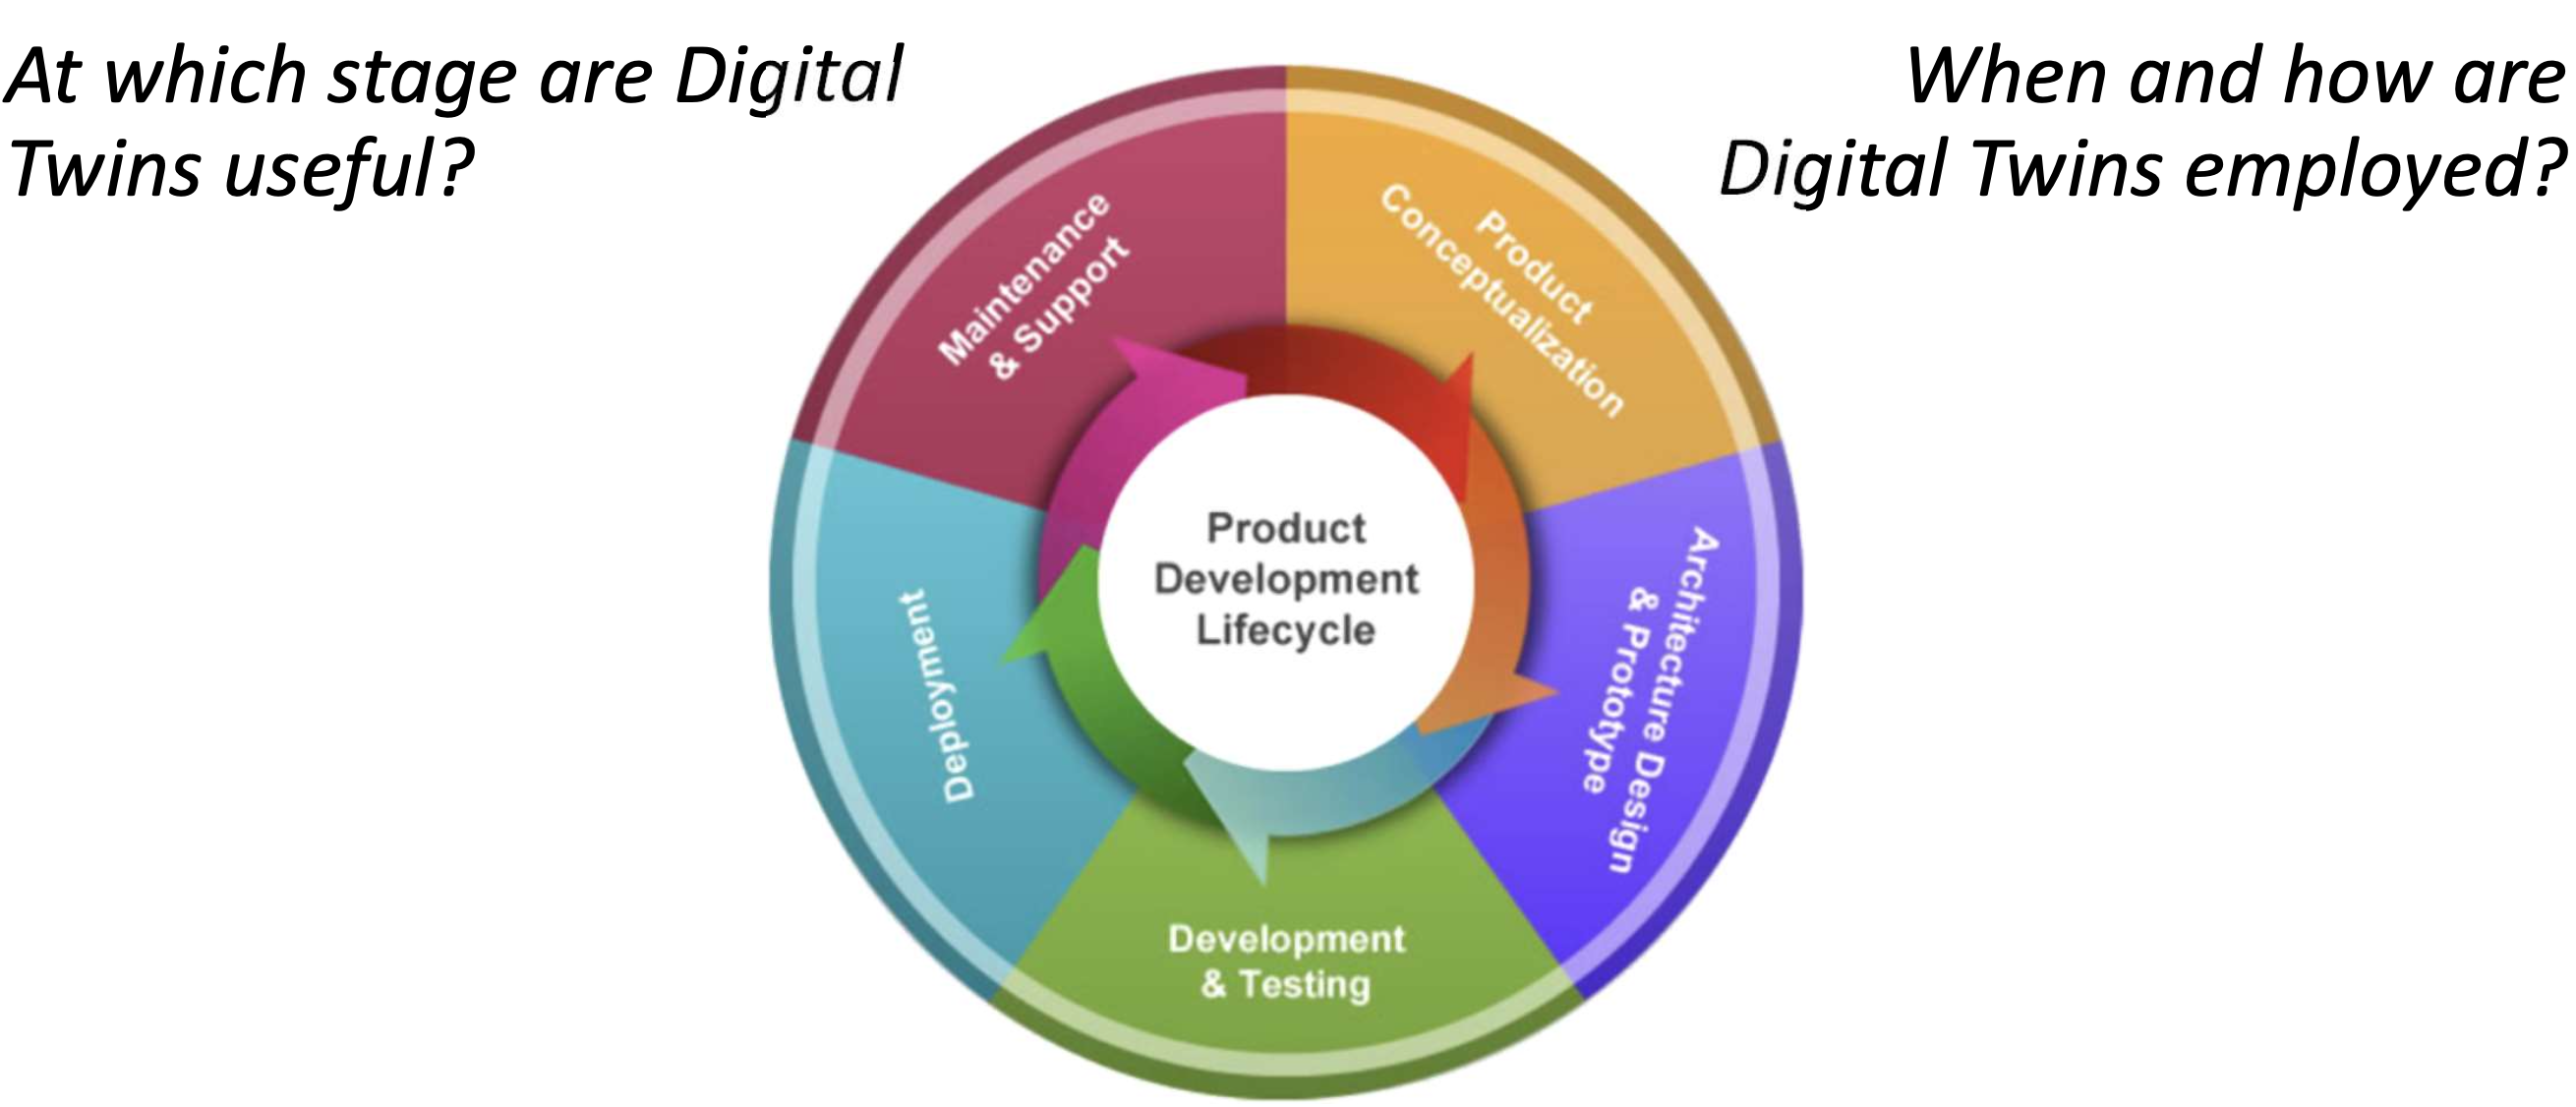
\includegraphics[width=0.9\linewidth]{assets/Screenshot 2026-01-16 at 17.18.37.png}
        \caption{Product development lifecycle;}\label{fig:app-intro1}
    \end{subfigure}
    \begin{subfigure}{0.9\linewidth}
        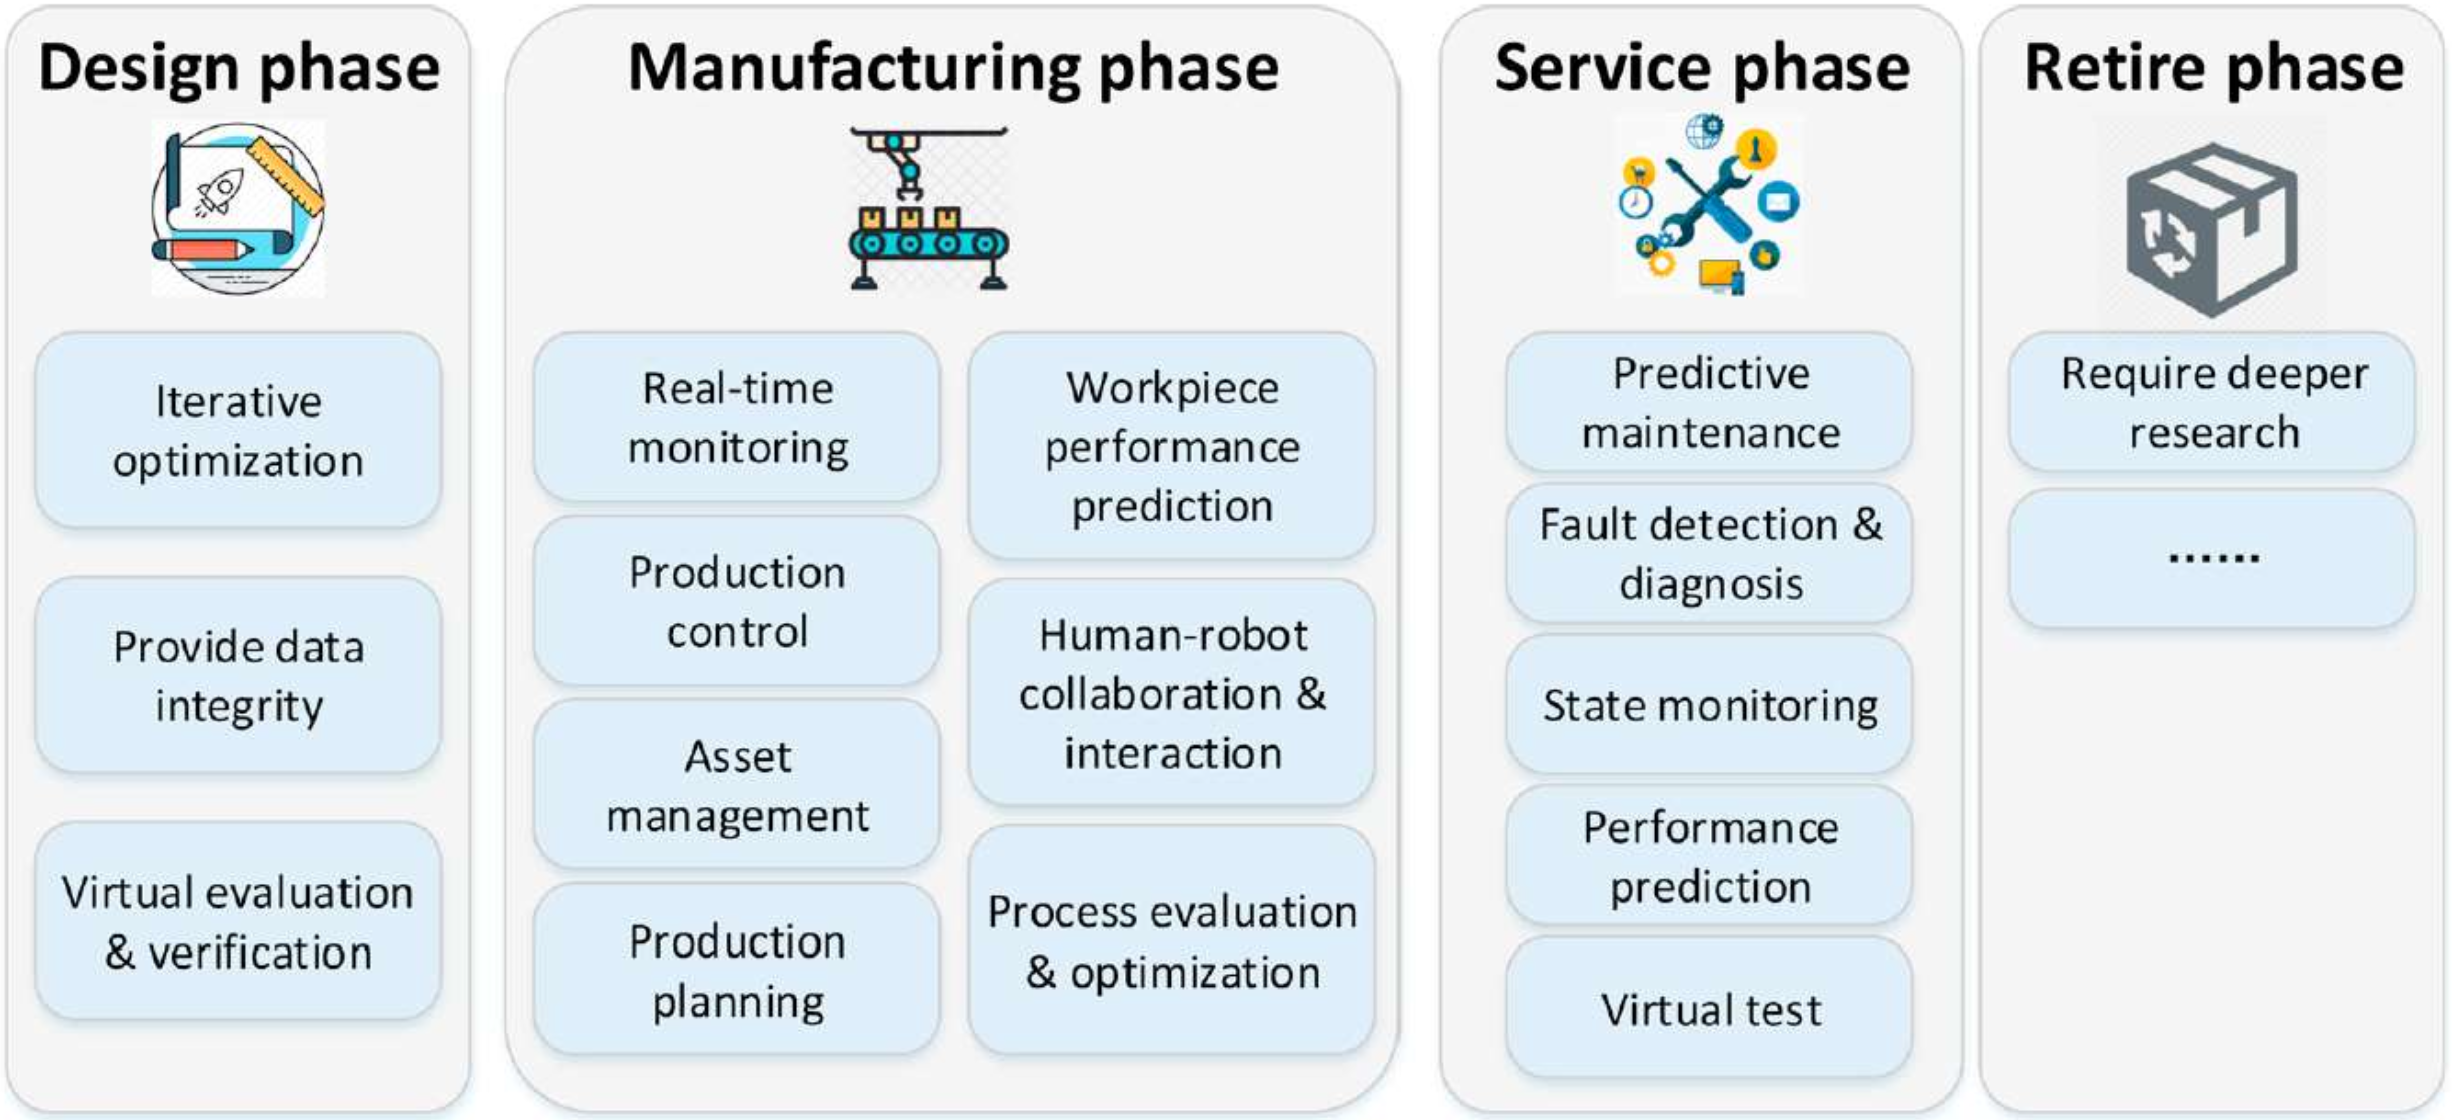
\includegraphics[width=0.9\linewidth]{assets/Screenshot 2026-01-16 at 17.20.17.png}
        \caption{Digital Twins in the product lifecycle;}\label{fig:app-intro2}
    \end{subfigure}
    \caption{Product lifecycle.}
\end{figure}

%
\section{Sfide principali}
Nonostante i benefici, l'adozione del DT affronta diversi ostacoli significativi:
\begin{itemize}
    \item Persone: Difficoltà nel comprendere il valore e uscire dalla ``comfort zone'', necessità di nuove competenze tecniche (modellazione, simulazione, data fusion);
    \item Tecnologia e Infrastrutture: Mancanza di soluzioni commerciali mature per la raccolta dati in tempo reale e limitazioni di connettività internet o performance dei sensori;
    \item Costi: Costruire un modello ad alta fedeltà e gestire l'elaborazione dati in tempo reale è costoso e richiede molto lavoro;
    \item Standardizzazione: Mancanza di standard per interfacce, modelli e protocolli che facilitino lo scambio dati;
    \item Cyber Security e Proprietà Intellettuale (IP): Necessità di proteggere dati sensibili, resistere ad attacchi sui sensori e tutelare i brevetti innovativi.
\end{itemize}

%
\section{Applicazioni industriali}
Nonostante le sfide, i Digital Twin hanno prospetti promettenti per il futuro (vedi figura \ref{fig:app-prospects}), vediamo allora come i DT possono essere applicati in settori specifici.
\begin{figure}
    \centering
    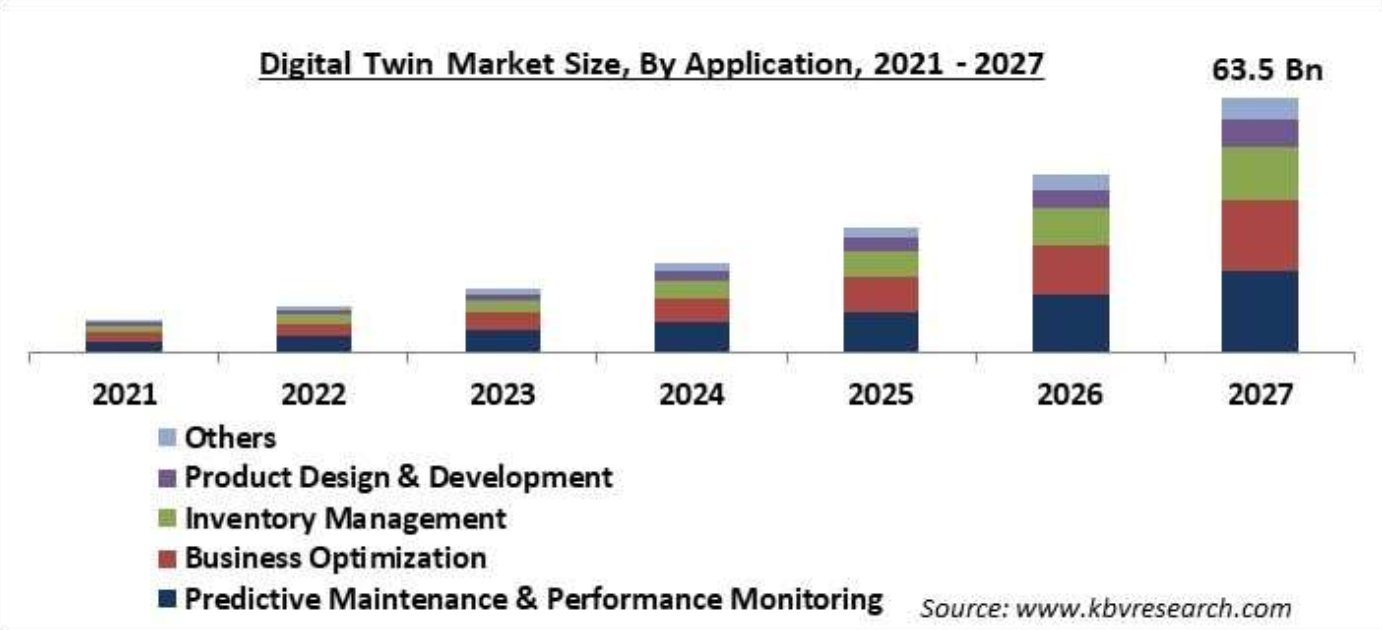
\includegraphics[width=0.9\linewidth]{assets/Screenshot 2026-01-16 at 17.27.13.png}
    \caption{}\label{fig:app-prospects}
\end{figure}
%
\subsection{Agricoltura}
Monitoraggio remoto delle colture, identificazione di parassiti e gestione della flotta macchinari. Viene citato l'uso di protocolli come LoRaWAN (basso consumo, lungo raggio) per creare reti locali di sensori che comunicano con il cloud.
%
\paragraph{LoraWAN} È un Low Power, Wide Area (LPWA) networking protocol, connette in modo wireless oggetti alimentati a batteria nel network. Vedi figura \ref{fig:app-lorawan}.
\begin{figure}
    \centering
    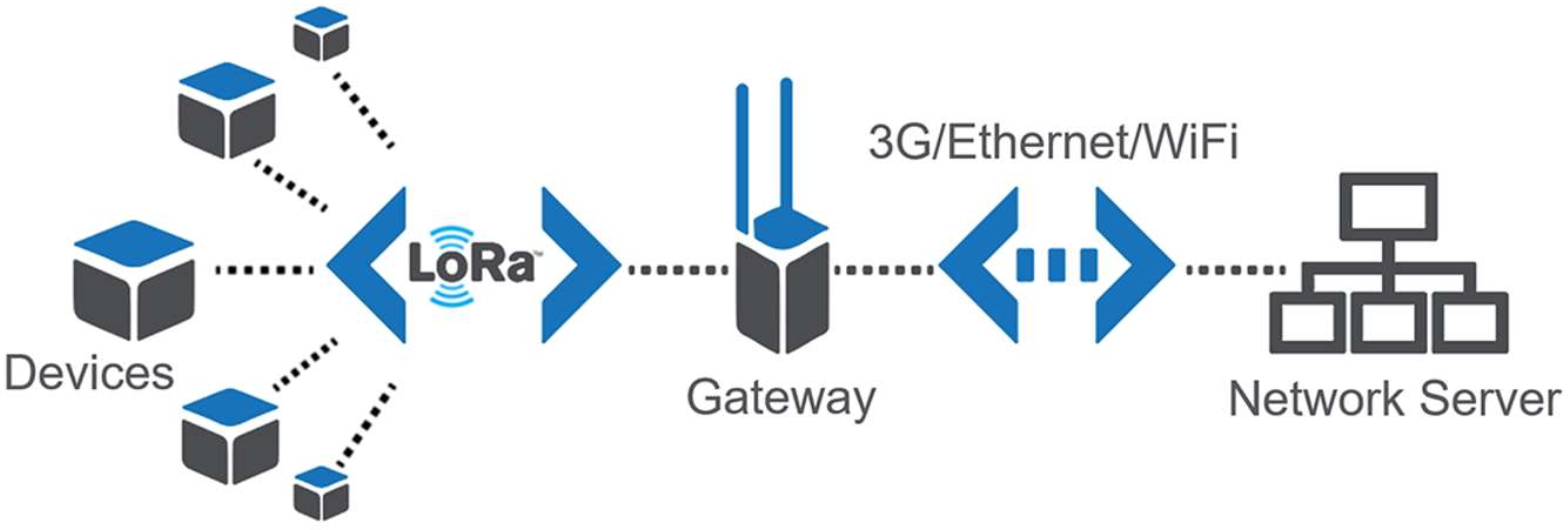
\includegraphics[width=0.9\linewidth]{assets/Screenshot 2026-01-16 at 17.30.46.png}
    \caption{}\label{fig:app-lorawan}
\end{figure}

%
\subsection{Aerospazio}
Settore pioniere (NASA, Airbus, Boeing). Usato per predire malfunzionamenti, strategie di manutenzione e simulare scenari per la sicurezza dell'equipaggio.
Il Digital Twin è stato adottato anche da produttori (es. Northrop Grumman, Airbus \dots) per supportare il processo di decision-making di prodotti non soddisfacenti e per trovare bottleneck nelle linee di produzione.
Vedi figure \ref{fig:app-aero_1} e \ref{fig:app-aero_2}.
\begin{figure}
    \centering
    \begin{subfigure}{0.45\linewidth}
        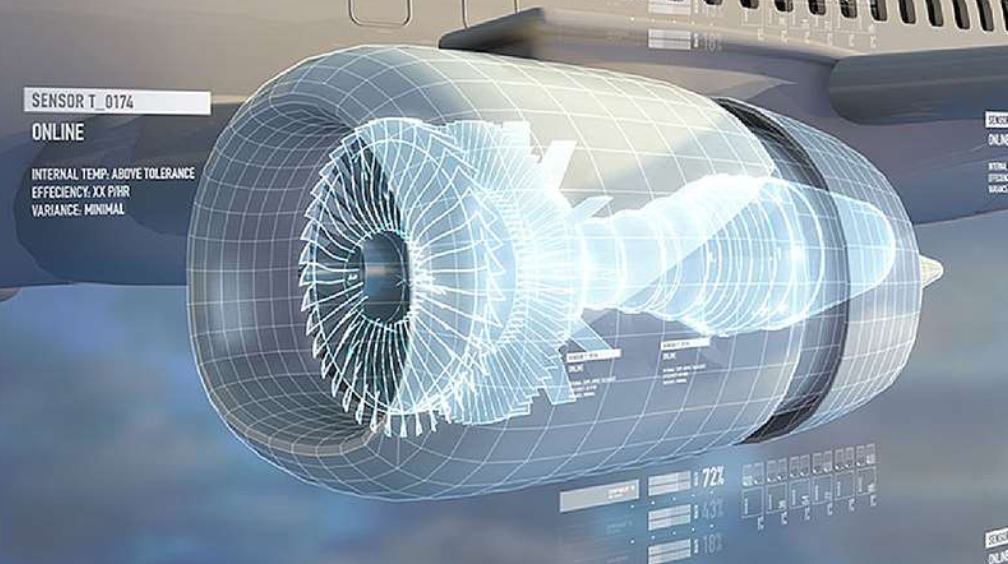
\includegraphics[width=\linewidth]{assets/Screenshot 2026-01-16 at 17.35.29.png}
        \caption{}\label{fig:app-aero_1}
    \end{subfigure}
    \begin{subfigure}{0.45\linewidth}
        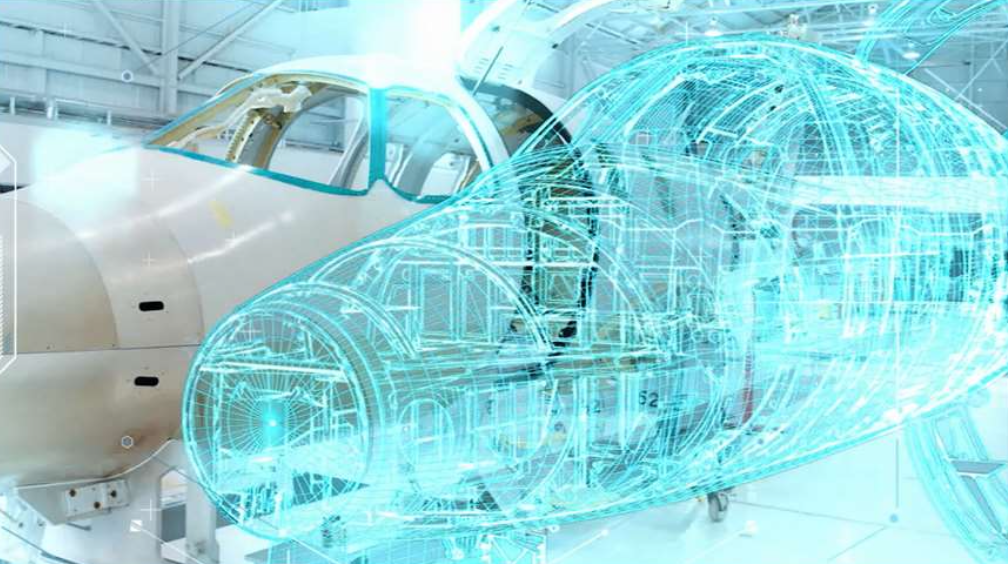
\includegraphics[width=\linewidth]{assets/Screenshot 2026-01-16 at 17.35.35.png}
        \caption{}\label{fig:app-aero_2}
    \end{subfigure}
    \caption{}\label{fig:app-aero}
\end{figure}

%
\subsection{Energia elettrica}
Possiamo vedere ad esempio la ``Digital Wind Farm'' di General Electric: ogni turbina ha un DT per ottimizzare la configurazione e aumentare la produzione energetica annuale. Vedi figura \ref{fig:app-eolico} per vedere una fantastica turbina eolica.
\begin{figure}
    \centering
    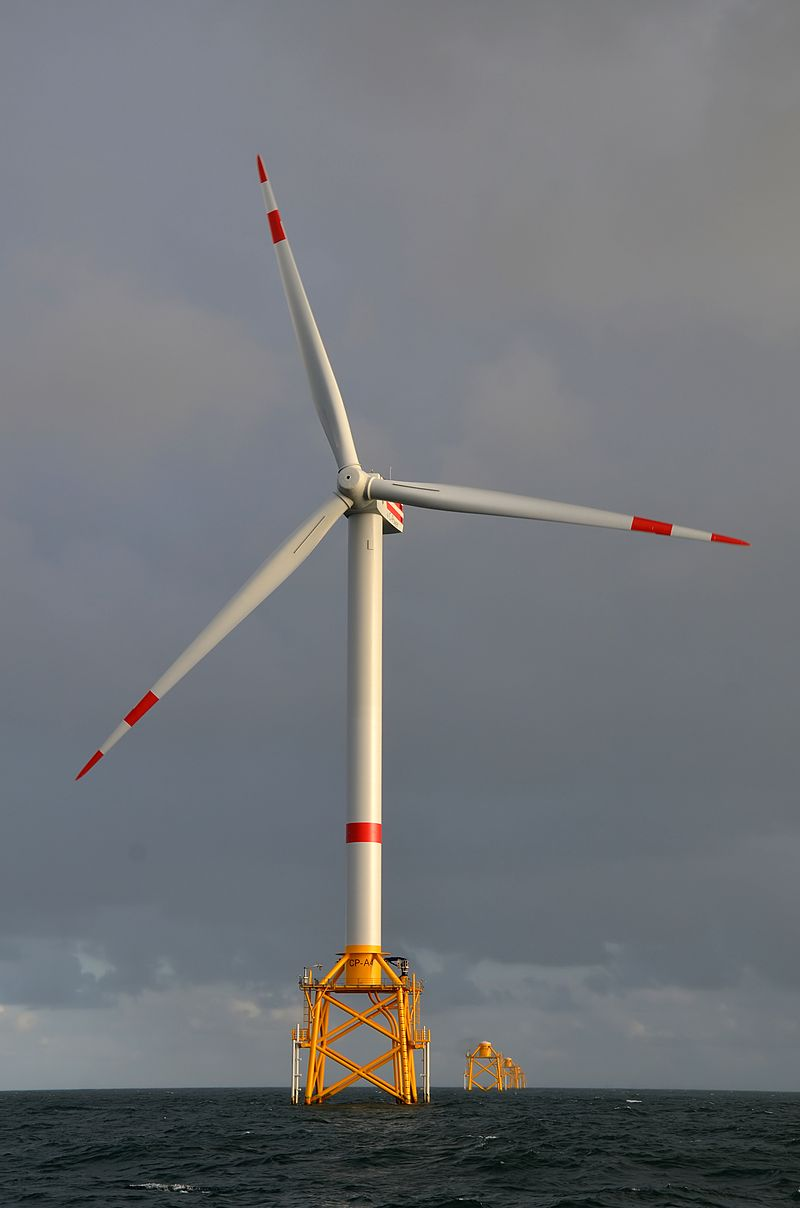
\includegraphics[width=0.25\linewidth]{assets/Una_turbina_eolica_nel_Mare_del_Nord.png}
    \caption{}\label{fig:app-eolico}
\end{figure}

%
\subsection{Automotive}
Fondamentale per la manutenzione predittiva e per simulare il comportamento del veicolo (o del motore) sotto condizioni specifiche per capire le cause dei guasti. Vedi figura \ref{fig:app-automotive}
\begin{figure}
    \centering
    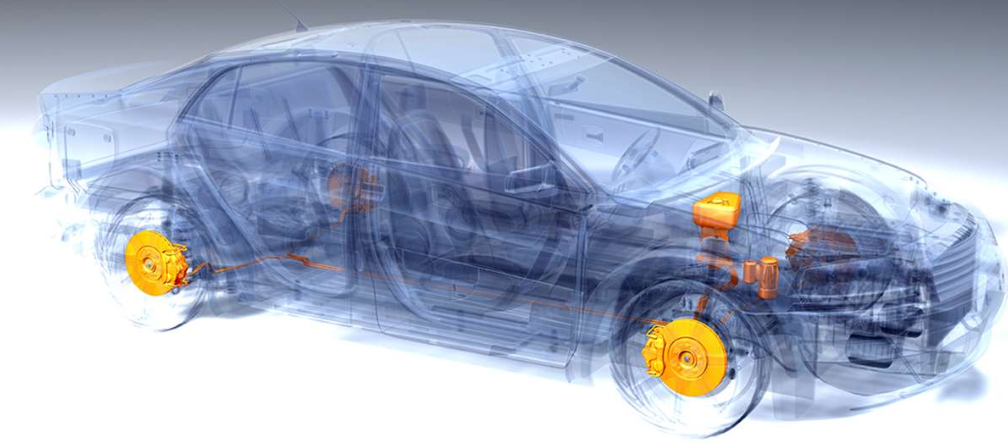
\includegraphics[width=0.9\linewidth]{assets/Screenshot 2026-01-16 at 17.51.41.png}
    \caption{}\label{fig:app-automotive}
\end{figure}

%
\subsection{Healthcare}
Dai ``gemelli digitali degli ospedali'' (gestione logistica, letti, staff \dots) alla medicina personalizzata (modelli di organi o dell'intero corpo umano per preparare chirurgie o testare trattamenti).

%
\section{Case study: Digital Twin di un braccio robotico}
%
\paragraph{Contesto} Presso l'\gls{icelab} al Politecnico di Torino, è stato sviluppato un DT per un braccio robotico industriale (KUKA) inserito in una linea di assemblaggio.
%
\paragraph{Obiettivo} Applicare degli algoritmi di Anomaly Detection per predire anomalie e guasti.
%

A riguardo le figure \ref{fig:app-casestudy1} e \ref{fig:app-casestudy2}.
\begin{figure}
    \centering
    \begin{subfigure}{0.45\linewidth}
        \centering
        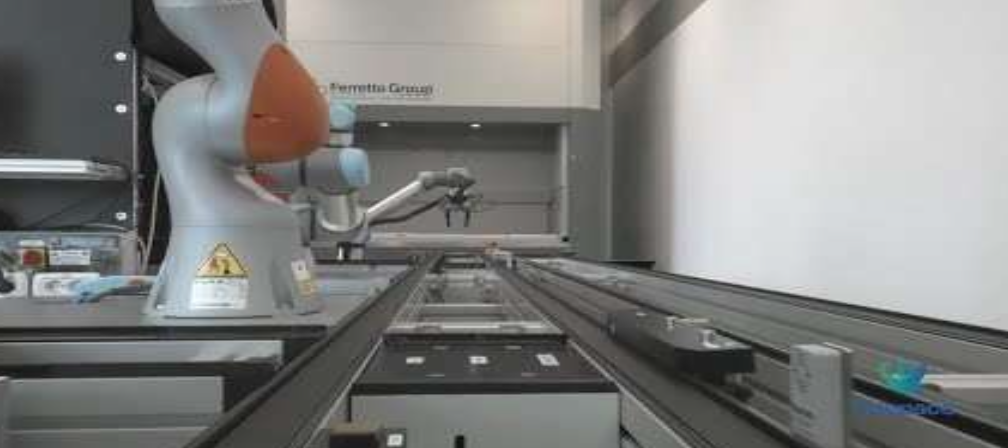
\includegraphics[width=\linewidth]{assets/Screenshot 2026-01-16 at 17.59.32.png}
        \caption{}\label{fig:app-casestudy1}
    \end{subfigure}
    \begin{subfigure}{0.45\linewidth}
        \centering
        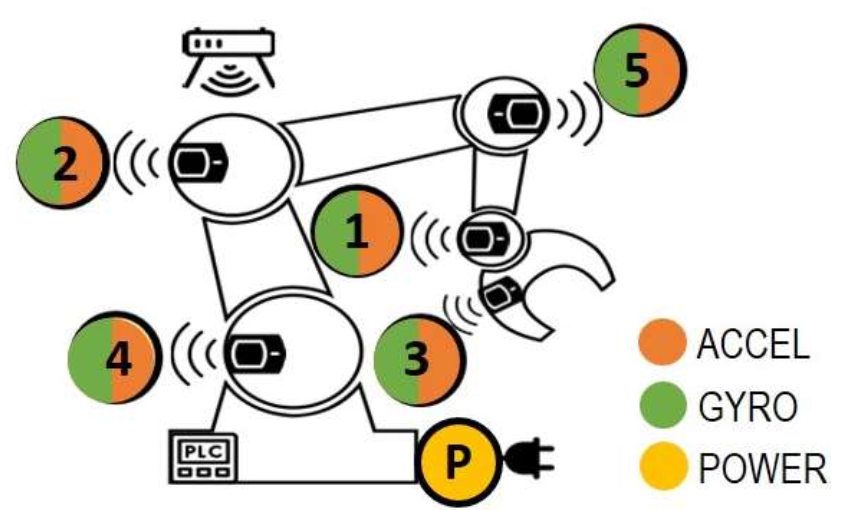
\includegraphics[width=\linewidth]{assets/Screenshot 2026-01-16 at 18.00.00.png}
        \caption{}\label{fig:app-casestudy2}
    \end{subfigure}
    \caption{}\label{fig:}
\end{figure}
\subsection{Data collection}
Il braccio è stato strumentato con 11 sensori aggiuntivi (5 giroscopi, 5 accelerometri, 1 sensore di potenza). I dati grezzi dei sensori vengono inviati a un gateway e poi ad un database (InfluxDB).